\begin{appendix}

\chapter{Current–Voltage Relationship of FETs--Mathematical Derivation}
\label{app:iv_FET}
\thispagestyle{plain}

This appendix gives the mathematical derivation of the ideal long-channel
field-effect-transistor current--voltage relations used in
Equation~\eqref{eq:fet_linear_current}. The derivation follows the standard
gradual-channel treatment of field-effect devices \cite{Neamen}. For consistency
with the $p$-channel convention used in the main text, all voltages and currents
are written as positive magnitudes.

The channel coordinate runs from the source at $x=0$ to the drain at $x=L$.
The local channel potential is $V(x)$, with
\begin{equation}
    V(0)=0,
    \qquad
    V(L)=V_\mathrm{DS}.
    \label{eq:app_fet_boundary_potentials}
\end{equation}
Within the gradual-channel approximation, the vertical gate field fixes the
local accumulated sheet charge, while the much smaller lateral field drives the
current. Above threshold, the mobile hole sheet charge is approximated by
\begin{equation}
    Q_\mathrm{p}(x)
    =C_\mathrm{i}\left[V_\mathrm{GS}-V_\mathrm{T}-V(x)\right],
    \label{eq:app_fet_sheet_charge}
\end{equation}
where $C_\mathrm{i}$ is the gate-insulator capacitance per unit area and
$V_\mathrm{T}$ is the threshold voltage. The expression is valid only where the
term in brackets is positive.

For constant mobility $\mu$, the drift current through a channel of width $W$ is
\begin{equation}
    I_\mathrm{D}
    =W\mu Q_\mathrm{p}(x)\frac{\mathrm{d}V}{\mathrm{d}x}.
    \label{eq:app_fet_local_current}
\end{equation}
Since the steady-state current is independent of $x$, substitution of
Equation~\eqref{eq:app_fet_sheet_charge} gives
\begin{equation}
    I_\mathrm{D}\,\mathrm{d}x
    =W\mu C_\mathrm{i}
    \left[V_\mathrm{GS}-V_\mathrm{T}-V\right]\mathrm{d}V.
    \label{eq:app_fet_separated_current}
\end{equation}
Integrating from source to drain yields
\begin{align}
    I_\mathrm{D}L
    &=W\mu C_\mathrm{i}
    \int_0^{V_\mathrm{DS}}
    \left[V_\mathrm{GS}-V_\mathrm{T}-V\right]\mathrm{d}V \\
    &=W\mu C_\mathrm{i}
    \left[
        \left(V_\mathrm{GS}-V_\mathrm{T}\right)V_\mathrm{DS}
        -\frac{V_\mathrm{DS}^2}{2}
    \right].
    \label{eq:app_fet_integrated_current}
\end{align}
Therefore the ideal linear-regime current is
\begin{equation}
    I_\mathrm{D}
    =\mu C_\mathrm{i}\frac{W}{L}
    \left[
        \left(V_\mathrm{GS}-V_\mathrm{T}\right)V_\mathrm{DS}
        -\frac{V_\mathrm{DS}^2}{2}
    \right],
    \qquad
    0\leq V_\mathrm{DS}<V_\mathrm{GS}-V_\mathrm{T}.
    \label{eq:app_fet_linear_current}
\end{equation}
For sufficiently small drain bias, the quadratic term can be neglected, giving
\begin{equation}
    I_\mathrm{D}
    \approx \mu C_\mathrm{i}\frac{W}{L}
    \left(V_\mathrm{GS}-V_\mathrm{T}\right)V_\mathrm{DS}.
    \label{eq:app_fet_small_vds_current}
\end{equation}
This limit shows that the accumulated channel behaves as a gate-controlled
resistor whose conductance is proportional to $V_\mathrm{GS}-V_\mathrm{T}$.

The channel reaches the ideal pinch-off condition when the charge at the drain
side vanishes,
\begin{equation}
    Q_\mathrm{p}(L)=0
    \quad\Rightarrow\quad
    V_\mathrm{DS,sat}=V_\mathrm{GS}-V_\mathrm{T}.
    \label{eq:app_fet_pinch_off_condition}
\end{equation}
Substitution of this condition into Equation~\eqref{eq:app_fet_linear_current}
gives the ideal saturation current,
\begin{equation}
    I_\mathrm{D,sat}
    =\frac{1}{2}\mu C_\mathrm{i}\frac{W}{L}
    \left(V_\mathrm{GS}-V_\mathrm{T}\right)^2.
    \label{eq:app_fet_saturation_current}
\end{equation}
In the ideal model this current is independent of further increases in
$V_\mathrm{DS}$. A finite output slope in real devices indicates additional
nonidealities such as channel-length modulation, field-dependent mobility,
contact resistance, or trap charging.

The usual mobility formulas follow directly from the two limiting forms. At
small fixed $V_\mathrm{DS}$,
\begin{equation}
    \mu_\mathrm{lin}
    =\frac{L}{W C_\mathrm{i}V_\mathrm{DS}}
    \frac{\mathrm{d}I_\mathrm{D}}{\mathrm{d}V_\mathrm{GS}}.
    \label{eq:app_fet_linear_mobility}
\end{equation}
In saturation,
\begin{equation}
    \sqrt{I_\mathrm{D,sat}}
    =\left(\frac{\mu C_\mathrm{i}W}{2L}\right)^{1/2}
    \left(V_\mathrm{GS}-V_\mathrm{T}\right),
    \label{eq:app_fet_sqrt_current}
\end{equation}
and therefore
\begin{equation}
    \mu_\mathrm{sat}
    =\frac{2L}{W C_\mathrm{i}}
    \left(
        \frac{\mathrm{d}\sqrt{I_\mathrm{D}}}
        {\mathrm{d}V_\mathrm{GS}}
    \right)^2.
    \label{eq:app_fet_saturation_mobility}
\end{equation}
These expressions are ideal model results. They give an intrinsic mobility only
when the assumptions of a uniform long channel, constant mobility, negligible
gate leakage, and negligible contact voltage loss are sufficiently fulfilled.
Otherwise the extracted value should be interpreted as an apparent mobility.

\chapter{Derivation of the Gated Van-der-Pauw Relation}
\label{app:gvdp_derivation}
\thispagestyle{plain}

This appendix derives the relation between the measured sheet conductance and
the gate-induced carrier density used in
Section~\ref{subsec:gvdp_density_mobility}. The derivation follows the
current-driven gated van der Pauw model introduced by Rolin et al.
\cite{Rolin2017GVDP}.

Consider the region between the two equipotential lines sensed by contacts 1 and
2. It can be represented by an equivalent field-effect channel with potentials
$V_1$ and $V_2$. Since contact 4 is the reference in this thesis,
$V_1=V_{14}$ and $V_2=V_{24}$. The local channel potential between these two
lines is denoted by $V(x)$, where $x$ is measured along the effective current
path from the line at $V_2$ to the line at $V_1$:
\begin{equation}
    V(0)=V_2,
    \qquad
    V(L)=V_1.
    \label{eq:app_gvdp_boundary_potentials}
\end{equation}
Within the gradual-channel approximation, the gate-induced sheet charge at this
position is controlled by the voltage difference between the gate and the local
semiconductor potential,
\begin{equation}
    Q_\mathrm{p}(x)
    =C_\mathrm{i}\left[V_\mathrm{G4}-V_\mathrm{T}-V(x)\right].
    \label{eq:app_gvdp_local_sheet_charge}
\end{equation}
For constant mobility, the drift current through an effective channel width $W$
is
\begin{equation}
    I_{34}
    =W\mu Q_\mathrm{p}(x)\frac{\mathrm{d}V}{\mathrm{d}x}.
    \label{eq:app_gvdp_local_current}
\end{equation}
Substituting Equation~\eqref{eq:app_gvdp_local_sheet_charge} into
Equation~\eqref{eq:app_gvdp_local_current} and separating variables gives
\begin{equation}
    I_{34}\,\mathrm{d}x
    =W\mu C_\mathrm{i}\left[V_\mathrm{G4}-V_\mathrm{T}-V\right]
    \mathrm{d}V.
    \label{eq:app_gvdp_separated_current}
\end{equation}
Because the same current crosses every equipotential line, the left-hand side can
be integrated from $x=0$ to $x=L$, while the potential on the right-hand side is
integrated from $V_2$ to $V_1$:
\begin{align}
    I_{34}L
    &=W\mu C_\mathrm{i}
    \int_{V_2}^{V_1}
    \left(V_\mathrm{G4}-V_\mathrm{T}-V\right)\mathrm{d}V \\
    &=W\mu C_\mathrm{i}
    \left[
        \left(V_\mathrm{G4}-V_\mathrm{T}\right)(V_1-V_2)
        -\frac{V_1^2-V_2^2}{2}
    \right].
    \label{eq:app_gvdp_integrated_current}
\end{align}
Dividing by $W$ and rewriting the bracket as a difference of squares gives
\begin{equation}
    I_{34}\frac{L}{W}
    =\frac{\mu C_\mathrm{i}}{2}
    \left[
    \left(V_\mathrm{G4}-V_\mathrm{T}-V_2\right)^2
    -
    \left(V_\mathrm{G4}-V_\mathrm{T}-V_1\right)^2
    \right].
    \label{eq:app_gvdp_drift_current}
\end{equation}
The effective geometrical ratio of a symmetric van der Pauw structure is
\begin{equation}
    \frac{L}{W}=\frac{\ln 2}{\pi}.
    \label{eq:app_gvdp_effective_geometry}
\end{equation}
Using the difference of two squares in
Equation~\eqref{eq:app_gvdp_drift_current} gives
\begin{align}
    I_{34}\frac{L}{W}
    & =\mu C_\mathrm{i}(V_1-V_2)
    \left[
    V_\mathrm{G4}-V_\mathrm{T}-\frac{V_1+V_2}{2}
    \right] \\
    & =\mu C_\mathrm{i}V_{12}
    \left(V_\mathrm{G4}-V_\mathrm{T}-V_\mathrm{C}\right),
    \label{eq:app_gvdp_expanded_current}
\end{align}
where
\begin{equation}
    V_{12}=V_1-V_2,
    \qquad
    V_\mathrm{C}=\frac{V_1+V_2}{2}.
    \label{eq:app_gvdp_voltage_definitions}
\end{equation}
The sheet conductance is defined by
\begin{equation}
    I_{34}\frac{L}{W}=\sigma_\mathrm{s}V_{12}.
    \label{eq:app_gvdp_sheet_ohm_law}
\end{equation}
Equating Equations~\eqref{eq:app_gvdp_expanded_current} and
\eqref{eq:app_gvdp_sheet_ohm_law}, and cancelling $V_{12}$, yields
\begin{equation}
    \sigma_\mathrm{s}
    =\mu C_\mathrm{i}
    \left(V_\mathrm{G4}-V_\mathrm{C}-V_\mathrm{T}\right).
    \label{eq:app_gvdp_conductance_relation_signed}
\end{equation}
For a $p$-type accumulation layer, the magnitude is used,
\begin{equation}
    \sigma_\mathrm{s}
    =\mu C_\mathrm{i}
    \left|V_\mathrm{G4}-V_\mathrm{C}-V_\mathrm{T}\right|.
    \label{eq:app_gvdp_conductance_relation_magnitude}
\end{equation}
Since $\sigma_\mathrm{s}=q n_\mathrm{2D}\mu$, comparison with
Equation~\eqref{eq:app_gvdp_conductance_relation_signed} gives the signed sheet
carrier density
\begin{equation}
    n_\mathrm{2D}
    =\frac{C_\mathrm{i}}{q}
    \left(V_\mathrm{G4}-V_\mathrm{C}-V_\mathrm{T}\right),
    \label{eq:app_gvdp_carrier_density}
\end{equation}
while the positive hole number density is the magnitude of this expression.
Differentiation of
Equation~\eqref{eq:app_gvdp_conductance_relation_magnitude} with respect to the
internal gate voltage gives
\begin{equation}
    \mu
    =\frac{1}{C_\mathrm{i}}
    \left|
    \frac{\mathrm{d}\sigma_\mathrm{s}}
    {\mathrm{d}(V_\mathrm{G4}-V_\mathrm{C})}
    \right|,
    \label{eq:app_gvdp_mobility_slope}
\end{equation}
provided that the mobility is approximately independent of gate voltage over
the fitted interval. The derivation also shows directly why
$V_\mathrm{C}$ must be subtracted: the accumulation charge is controlled by the
voltage between the gate and the local semiconductor sheet, not by the gate
voltage relative to the grounded current contact alone.

%%%%%%%%%%%%%%%%%%%%%%%%%%%%%%%%%%%%%%%%
%%%%%%%%%%%%%%%%%%%%%%%%%%%%%%%%%%%%%%%%



\chapter{Numerical Simulation of the Van der Pauw Configuration}
\label{app:vdp_simulation}
\thispagestyle{plain}

This appendix summarizes the numerical procedure used to calculate the
potential and hole-density maps shown in the theory chapter. The calculation is
only a qualitative visualization of lateral electrostatics in a four-contact
van der Pauw geometry. It is not used to extract a mobility, sheet density, or
representative channel potential. Therefore the experimental correction
$V_\mathrm{C}$ is not a relevant output of this numerical appendix; the voltage
probe contacts are included only as passive geometrical markers.

The semiconductor is represented by a square two-dimensional grid with spacing
$h$. The biased contacts impose fixed electrostatic potentials, while insulating
outer boundaries satisfy zero-normal-field conditions. The local hole density is
approximated by a Boltzmann relation,
\begin{equation}
    p_{i,j}
    =N_\mathrm{v}
    \exp\left[-\frac{F_{i,j}+e\phi_{i,j}}{k_\mathrm{B}T}\right],
    \label{eq:vdp_sim_compact_density}
\end{equation}
where $\phi_{i,j}$ is the electrostatic potential and $F_{i,j}$ is the local
hole quasi-Fermi energy. The applied gate bias is not solved explicitly in this
two-dimensional model; for a chosen $V_\mathrm{G4}$ it is represented by the
fixed background charge density in Poisson's equation~\cite{Stodtmann2012OrganicSimulation,Darwish2020DriftDiffusionOFET},
\begin{equation}
    \nabla^2\phi=-\frac{\rho}{\varepsilon},
    \qquad
    \rho=e(p-N_\mathrm{A}),
    \label{eq:vdp_sim_poisson_compact}
\end{equation}
Here $N_\mathrm{A}$ denotes this effective background charge density. In a full device model it may depend on the selected gate voltage, but in the present simplified Poisson solve it is held constant during the iteration.

For an interior grid point, the finite-difference form of
Equation~\eqref{eq:vdp_sim_poisson_compact} is
\begin{equation}
    \frac{
        \phi_{i+1,j}+\phi_{i-1,j}+\phi_{i,j+1}+\phi_{i,j-1}-4\phi_{i,j}
    }{h^2}
    =-\frac{\rho_{i,j}}{\varepsilon}.
    \label{eq:vdp_sim_discrete_poisson}
\end{equation}
Solving this expression for the central value gives the Jacobi update candidate~\cite{hackbusch2016iterative},
\begin{equation}
    \phi^{*}_{i,j}
    =\frac{1}{4}\left(
        \phi^{(k)}_{i+1,j}+\phi^{(k)}_{i-1,j}
        +\phi^{(k)}_{i,j+1}+\phi^{(k)}_{i,j-1}
        +\frac{h^2\rho^{(k)}_{i,j}}{\varepsilon}
    \right).
    \label{eq:vdp_sim_jacobi_candidate}
\end{equation}
Because $p$ depends exponentially on $\phi$, direct replacement can be unstable.
The update is therefore under-relaxed, a standard stabilization strategy for nonlinear fixed-point iterations~\cite{hackbusch2016iterative},
\begin{equation}
    \phi^{(k+1)}_{i,j}
    =(1-\alpha_\phi)\phi^{(k)}_{i,j}
    +\alpha_\phi\phi^{*}_{i,j},
    \label{eq:vdp_sim_relaxed_poisson_update}
\end{equation}
with $0<\alpha_\phi<1$. After each update, the contact potentials and insulating
boundary conditions are reapplied.

The iterative solution is performed as follows. First, an initial potential
$\phi^{(0)}$ satisfying the contact voltages is chosen. The hole density and
space charge are then calculated from
Equations~\eqref{eq:vdp_sim_compact_density} and
\eqref{eq:vdp_sim_poisson_compact}. Next, all interior potentials are updated
with Equations~\eqref{eq:vdp_sim_jacobi_candidate} and
\eqref{eq:vdp_sim_relaxed_poisson_update}. This sequence is repeated until the
relative change
\begin{equation}
    \eta^{(k)}
    =\frac{\max_{i,j}|\phi^{(k+1)}_{i,j}-\phi^{(k)}_{i,j}|}
    {\max\left(\max_{i,j}|\phi^{(k)}_{i,j}|,10^{-30}\right)}
    \label{eq:vdp_sim_convergence_compact}
\end{equation}
falls below the selected tolerance. If current streamlines are required, the
quasi-Fermi field is updated in a second conservative step from
$\nabla\cdot(p\nabla F)=0$, but the central electrostatic part of the calculation
is the iterative Poisson solve described above.

\begin{figure}[htbp]
    \centering
    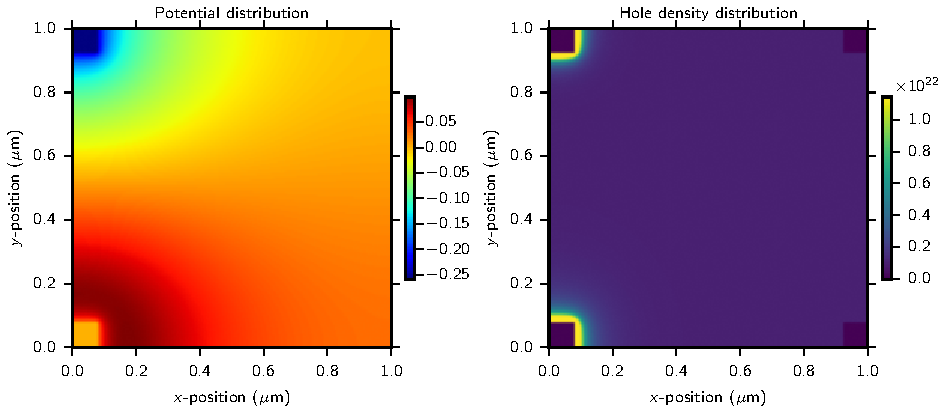
\includegraphics[width=0.88\textwidth]
        {figures/gvdP-simulation.pdf}
    \caption[Simulated potential and hole-density distributions]
    {Calculated potential and hole-density distributions in the gated van der
    Pauw structure. The potential map is obtained by iteratively solving
    Poisson's equation on the two-dimensional grid with fixed contact
    potentials and insulating outer boundaries. The hole-density map is then
    calculated from the local electrochemical energy and shows hole
    accumulation near the current-carrying contacts.}
    \label{fig:vdp_sim_results}
\end{figure}

Figure~\ref{fig:vdp_sim_results} illustrates the result of this iterative
procedure. The potential is not uniform across the semiconductor sheet because
the imposed contact potentials and insulating edges force the field lines to
spread through the two-dimensional domain. Since the hole density is coupled to
this potential through Equation~\eqref{eq:vdp_sim_compact_density}, the density
also becomes spatially nonuniform and is enhanced near the current-carrying
contacts. The model remains idealized: it uses constant material parameters,
Boltzmann statistics, simplified contact boundary conditions, and no explicit
vertical gate-stack electrostatics. It should therefore be interpreted as a
visualization of the iterative electrostatic solution rather than a quantitative
prediction of the experimental mobility or carrier concentration.

\end{appendix}
